\documentclass[sigconf, anonymous]{acmart}
\usepackage{graphics}
\usepackage{amsmath}
\usepackage{multirow}
% \usepackage[affil-it]{authblk}

\newcommand{\ToDo}[1]{{\noindent \color{blue}{\##1}}}
\newcommand{\highlighto}[1]{{\color{orange}{#1}}}
\newcommand{\highlightr}[1]{{\color{red}{#1}}}
\newcommand{\highlightg}[1]{{\color{green}{#1}}}

\newcommand{\FW}[1]{{\noindent \color{red}{#1}}}
\newcommand{\Alfred}[1]{\textcolor{red}{[Alfred: #1]}}

% \fancyhf{} % Remove fancy page headers 

% \fancyhead[C]{Anonymous submission \#9999 to ACM CCS 2017} % TODO: replace 9999 with your paper number
\fancyfoot[C]{\thepage}

\setcopyright{none} % No copyright notice required for submissions
% \acmConference[Anonymous Submission to ACM CCS 2017]{ACM Conference on Computer and Communications Security}{Due 19 May 2017}{Dallas, Texas}
% \acmYear{2020}

\settopmatter{printacmref=false, printccs=true, printfolios=true} % We want page numbers on submissions
\renewcommand\footnotetextcopyrightpermission[1]{}
% \pagestyle{plain}

\begin{document}
\fancyhead{}

% \title{AttacKG: Practical CTI Report Parsing \& Threat Intelligence KG Building}
\title{AttacKG: Extract Provenance Graph-level Attack Variants from Cyber Threat Intelligence Reports} % Identify in

\vspace{-0.1in}
\author{Zhenyuan Li} % end author
\affiliation{\institution{Zhejiang University, China}}

\begin{abstract}

Threat intelligence are widely adopt in both academia and industry. However, the existing, widely used threat intelligence formats are quite crude \cite{Li2019}, hard to defent well-organized APT attacks. Thus, in this paper, we proposed a new graph-based threat intelligence framework.

Another problem that needs to be addressed is the extensive collection of threat intelligence. To address this problem, we ...

\end{abstract}

% TODO: replace this section with code generated by the tool at https://dl.acm.org/ccs.cfm
\begin{CCSXML}
<ccs2012>
<concept>
<concept_id>10002978.10003029.10011703</concept_id>
<concept_desc>Security and privacy~Usability in security and privacy</concept_desc>
<concept_significance>500</concept_significance>
</concept>
</ccs2012>
\end{CCSXML}

% \ccsdesc{Security and privacy~Use https://dl.acm.org/ccs.cfm to generate actual concepts section for your paper}

% \keywords{mimicry attack; provenance graph; threat detection; evasion} % TODO: replace with your keywords

\maketitle

\section{Introduction}
\label{sec:introduction}

\subsection{Background}

\ToDo{1 Cyber attacks are diversifying.}

\ToDo{2 Threat intelligence and threat reports are helpful tools}

Provenance graph as a threat representation tool are already widely studied and adopted \cite{li2021}. With provenance graph, security analyzers are able to encode system execution history into graphs. Thus provenance graph contain rich semantic information. However, there are still a gap between provenance graphs and human understandable information. Poirot \cite{Milajerdi2019} try to solve this problem by involve TTPs and kill chain proposed by MITRE \cite{}.

\ToDo{3 Provenance graph are widely-used and recongnized threat representation approach.}

\subsection{Related Works}

\ToDo{1 Compare with existing automated threat intelligence collection works.}

\ToDo{2 How our work support provenance graph-based threat detection.}

\subsection{Our work}

\ToDo{1 Extracting incomplete attack graph from single CTI report.}

\ToDo{2 Delineating behavioural and clustering analysis.}

\ToDo{3 Implement applicaitons.}

\subsection{Contribution}

\ToDo{1 New threat intelligence representation approach.}

\ToDo{2 Automated threat intelligence collection and management system.}

\ToDo{3 Collected a large amount of threat intelligence and done a through analysis by real-word application.}

\ToDo{4 We provided a open attack dataset.}


\begin{figure}
    \centering
    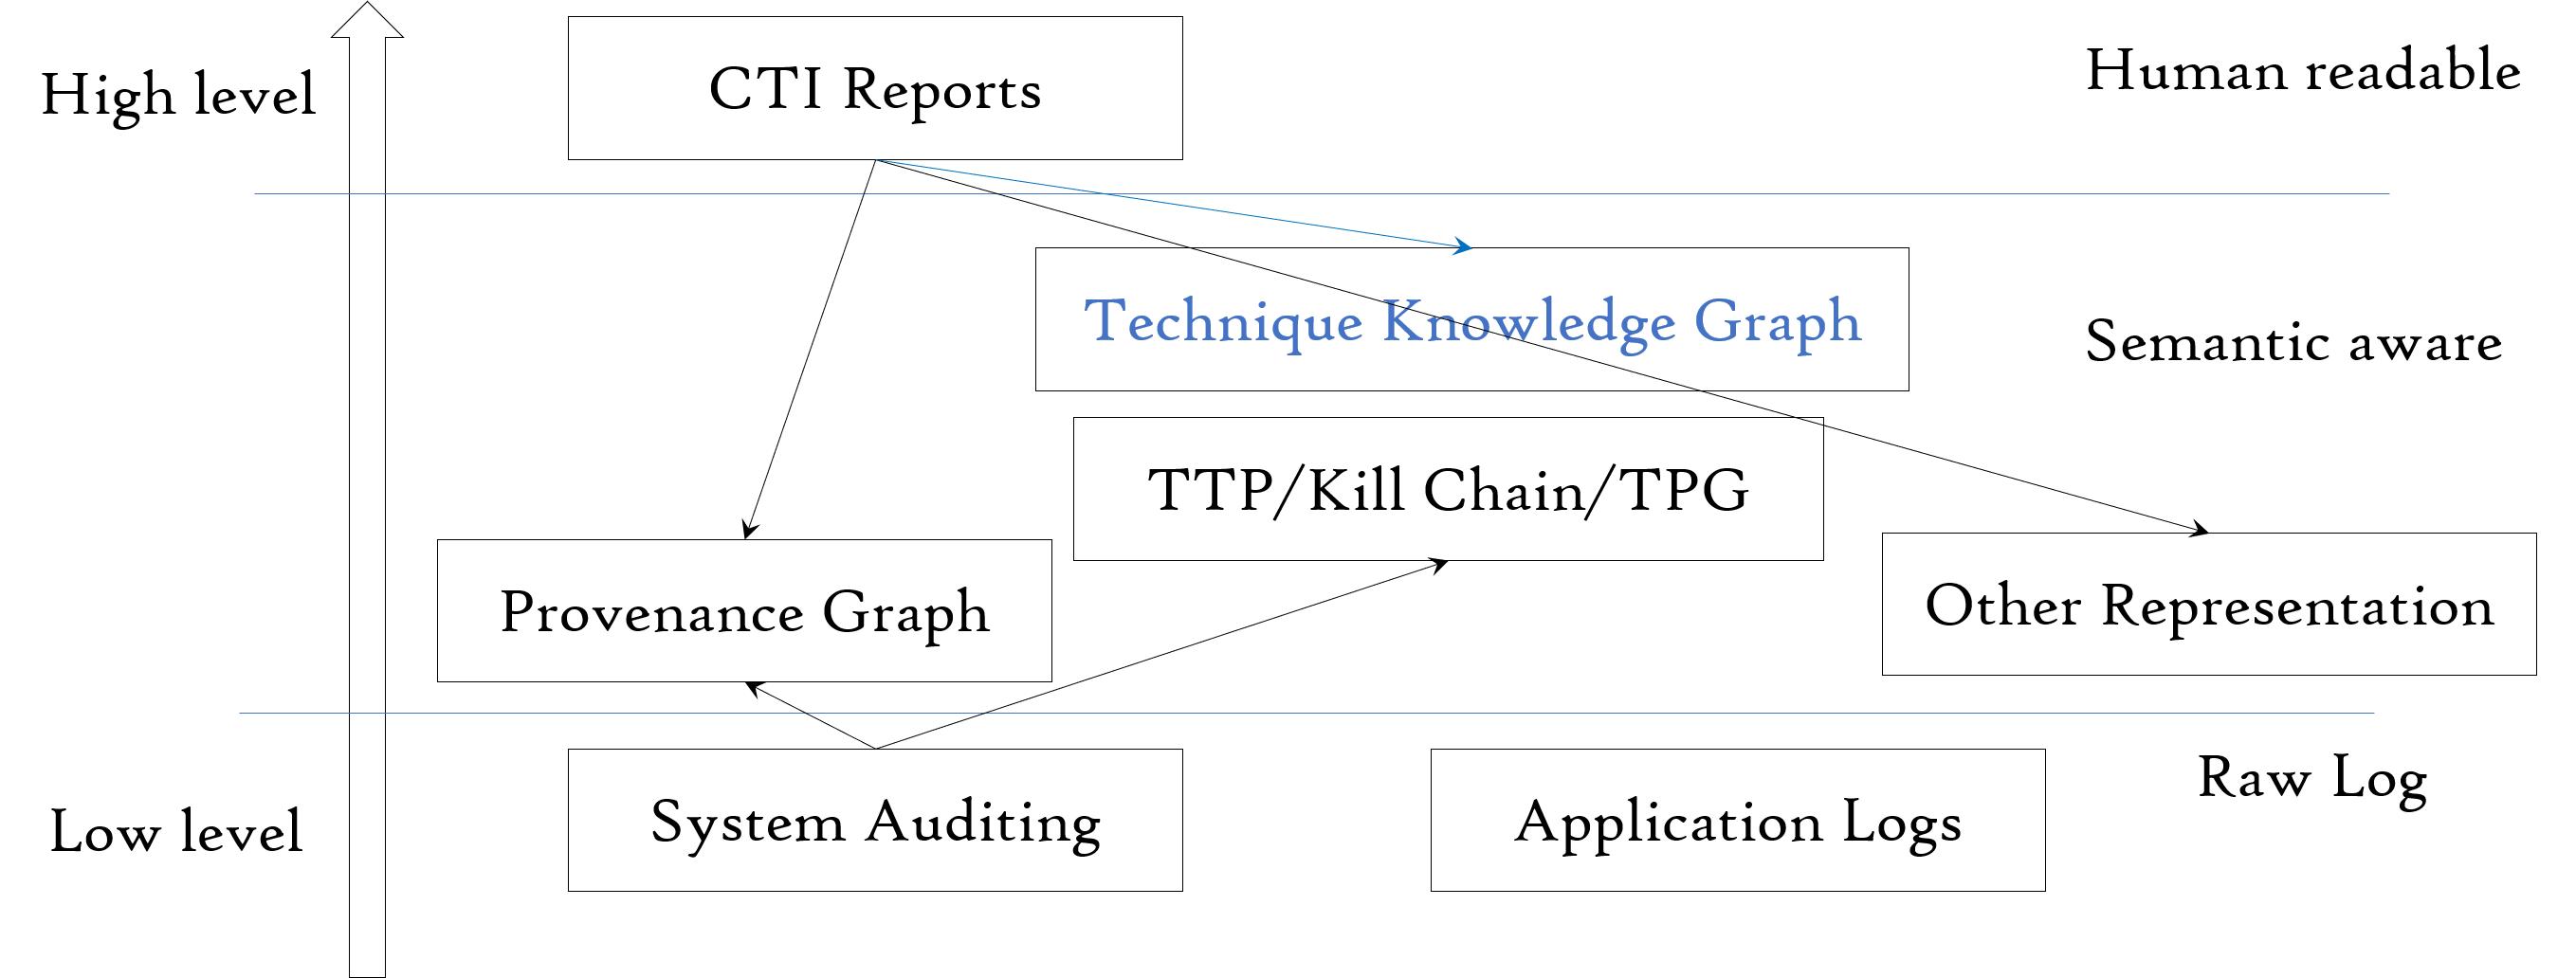
\includegraphics[width=3.5in]{Image/representation.png}
    \caption{Different Representation of Cyber Attacks.}
    \label{fig:representation}
\end{figure}

\section{Related Work}
\label{sec:relatedworks}

\subsection{Threat Intelligence}

Threat intelligence are widely adopt in both academia and industry. \cite{Berady2021,Michael2021} 

\subsection{Extract threat intelligence from unstructured CTI reports}

Existing works try to extract IoC \cite{Liao}, TTPs \cite{Husari2017}, Attack Chains \cite{Zhu2018}, Attack Graph \cite{Gao} from unstructed TI. Most recent works tend to extract more detailed and structure information. Ideal CTI should be general to cover more attack cases while detailed to avoid FP. To strike a balance, we need to correlate related attack descriptions and construct a better one.

However, single CTI report cannot provide 

\subsection{Modeling the cyber threat intelligence (Knowledge graphs for security purpose)}

\cite{Gao2020,Zhao2020} try to model and quantify the underlying relationship among heterogeneous IoCs (Attackers, Device, Platform, Vulnerability, File, Type). These works do not include information about how these IoCs work together (PG), and leave lots of details.

\subsection{Threat detection and forensic (Adopt graphs to represent cyber attacks)}

\cite{Milajerdi2019}, etc. can adopt threat intelligence extracted by our system. Accurate and general attack description can ensure detection efficiency and accuracy.
\section{Background}
\label{sec:background}

\subsection{Three granularity of variant for PG}

\ToDo{1 Different combination of attack techniques.}

\ToDo{2 Different mplementation of attack techniques.}

\ToDo{3 Different option for attack nodes.}
\cite{Michael2021} \cite{Kurogome2019}

\subsection{Problem statement}

CTI reports contain rich information needed by detection and analyzer. However, existing reports analysis work focus only on the reports itself, leave out lots of useful information. We propose to adopt TTPs knowledge and Technique/Tactic Knowledge Graph(TKG) to organize the knowledge extracted from reports. And generate more useful attack descriptions.

On the one hand, current CTI sources focus on naïve IoCs, such as bad IPs, malware hashes, etc., without much high-level semantic. Such CTI are neither general nor reliable. \cite{Li2019} On the other hand, unstructed threat whitepapers are vague. – We need new CTI standards. 

On the other hand, effective(fast) and efficient(accuracy) detection require accurate attack description. State-of-the-art work rely on manual analysis \cite{Milajerdi2019} which is difficult to expand. – We need more and automated CTI. 

\subsection{Challenges}

\ToDo{C1. How to extract Techniques from Natural-Language CTI? – \S\ref{sub_sec:nlp_parser}}
% Contribution 1: Automated report parsing. S: TTPs templates (knowledge base) vs. Patterns in CTI (NLP)

C1-1. Unstructured Threat Whitepapers Are Vague: 

Vague nodes: Lack of explicit node identification; Vague subject: 

Vague edges: An operation may corresponds to a series of edges in PG

C1-2. How to find technique dependencies? (Sometimes)
S: Employ System Entity/Report/self-defined tags(TCP sockets) as connections

\ToDo{C2. How to integrate multiple CTI reports? – Contribution 2: Building attack Technique Knowledge Graph. -\S\ref{sub_sec:TKG_update}}

Observations:

1. A single report most likely covers a fragment of an APT attack?

2.Different reports may conflict due to variant malwares


\ToDo{C3. How to use the TKG?  - What basic function we need to implement on TKG? -\S\ref{sec:case_study}}

\section{System Design}
\label{sec:system_design}
\section{Implementation}
\label{sec:Implementation}
\section{Evaluation}
\label{sec:evaluation}

Our evaluation aim to answer the following research questions:

\ToDo{RQ1: How accurate is AKG in extracting threat behaviors from CTI report? -- \S\ref{sub_sec:nlp_parser}}

\ToDo{RQ2: How accurate is AKG in matching (\textbf{and finding}) attack variant in different CTI report? -- \S\ref{sub_sec:matching}

We can adopt MITRE reference to test our technique identification accuracy.

\textbf{Accuracy + Efficiency} \textit{node set matching vs ordered node set matching vs graph( = node set + edge set) matching}

\textbf{Accuracy} \textit{template from MITRE vs template from (MITRE + reports)}
}

\section{Discussion}
\label{sec:discussion}


% \section{Conclusions}
% In this poster, we proposed a mimicry attack approach against provenance graph. With such attack, we are able to...

% We provide a preliminary idea about why one-hop-based anomaly analysis is unreliable. 

% In the following work, we will research...

% Longer attack chain, Evasion against 

\appendix

\section{Technique Attack Graph Extracted from CTI Reports}
\section{Attack Variants Extracted from CTI Reports}


\begin{acks}
We would like to thank the anonymous reviewers for providing valuable feedback on our work. This work is supported by the Zhejiang Lab’s International Talent Fund for Young Professionals.
\end{acks}


\vspace{-0.04in}
% \bibliographystyle{ACM-Reference-Format}
\bibliographystyle{acm}
\bibliography{AttacKG}

\end{document}
